% ================================================================
% FHE Hardware Accelerator — Optimisation 1 Report
% Elimination of Internal Ciphertext Buffer in hash_verifier
% Compile: pdflatex report_optimisation1.tex (twice for references)
% ================================================================
\documentclass[12pt, a4paper]{article}

\usepackage{amsmath, amssymb}
\usepackage{booktabs}
\usepackage{graphicx}
\usepackage{xcolor}
\usepackage{listings}
\usepackage{tikz}
\usetikzlibrary{arrows.meta, positioning, shapes, fit, calc}
\usepackage{hyperref}
\usepackage{geometry}
\usepackage{caption}
\usepackage{subcaption}
\usepackage{array}
\usepackage{multirow}

\geometry{margin=2.5cm}

\definecolor{codebg}{rgb}{0.97,0.97,0.97}
\definecolor{codegreen}{rgb}{0.0,0.45,0.0}
\definecolor{codegray}{rgb}{0.45,0.45,0.45}
\definecolor{codeblue}{rgb}{0.0,0.0,0.75}
\definecolor{codepurple}{rgb}{0.55,0.0,0.55}

\lstdefinelanguage{Verilog}{
  keywords={module, endmodule, input, output, wire, reg, always, posedge,
            begin, end, case, endcase, if, else, assign, parameter,
            localparam, integer, task, endtask, for, default},
  keywordstyle=\color{codeblue}\bfseries,
  comment=[l]{//},
  commentstyle=\color{codegray}\itshape,
  stringstyle=\color{codegreen},
  sensitive=true
}

\lstset{
  language=Verilog,
  backgroundcolor=\color{codebg},
  basicstyle=\ttfamily\small,
  breaklines=true,
  frame=single,
  numbers=left,
  numberstyle=\tiny\color{codegray},
  numbersep=6pt,
  tabsize=4,
  showstringspaces=false,
  captionpos=b
}

% ── Title ──────────────────────────────────────────────────────
\title{
  \textbf{FHE Hardware Accelerator}\\[0.4em]
  \large Optimisation 1: Elimination of Internal Ciphertext Buffer\\
  in the \texttt{hash\_verifier} Module
}
\author{FHE Hardware Project}
\date{\today}

% ================================================================
\begin{document}
\maketitle
\tableofcontents
\newpage

% ================================================================
\section{Background}
\label{sec:background}

This report documents the first hardware optimisation applied to an
FPGA-accelerated Fully Homomorphic Encryption (FHE) hash verifier,
targeting the Xilinx Artix-7 \textbf{xc7a200t} device.

\subsection{System Overview}

The system accelerates a homomorphic hash-based ciphertext verification
scheme based on the BV homomorphic encryption scheme over the
negacyclic polynomial ring $\mathbb{Z}_q[X]/(X^N+1)$.

Key parameters are listed in Table~\ref{tab:params}.

\begin{table}[h]
\centering
\begin{tabular}{lll}
\toprule
\textbf{Parameter} & \textbf{Value} & \textbf{Description} \\
\midrule
$N$ & $8192 = 2^{13}$ & Polynomial degree \\
\texttt{Q\_WIDTH} & 40 bits & Coefficient modulus bit-width \\
$q$ & $883{,}949{,}569$ & NTT-friendly prime ($q \equiv 1 \bmod 2N$) \\
\texttt{CT\_SIZE} & 3 & Maximum ciphertext components \\
Target device & xc7a200t & Xilinx Artix-7 FPGA \\
Available BRAM36 & 365 & On-chip block RAM tiles \\
\bottomrule
\end{tabular}
\caption{Design parameters.}
\label{tab:params}
\end{table}

\subsection{Ciphertext Structure}

In the BV scheme, a ciphertext is a \emph{tuple of polynomials}
(components), not a single polynomial. A freshly encrypted ciphertext
has two components:
\[
  \mathbf{ct} = (c_0,\, c_1), \quad c_i \in \mathbb{Z}_q[X]/(X^N+1)
\]
Ciphertext multiplication grows the tuple length:
\[
  \mathbf{ct}_3 = \mathbf{ct}_1 \times \mathbf{ct}_2
  \;\Rightarrow\;
  \mathbf{ct}_3 = (e_0, e_1, e_2) \quad \text{(3 components)}
\]
Each component is a polynomial of $N=8192$ coefficients, each 40 bits
wide. Loading one component therefore requires $N$ write operations.

\subsection{Hash Verification Circuit}

The \texttt{hash\_verifier} module verifies the circuit
$\mathbf{c}_3 = \mathbf{c}_1 \cdot \mathbf{c}_2 + \mathbf{c}_2$
without decryption, using a ring homomorphism hash function
$H$ (Horner evaluation):
\[
  H(\mathbf{ct},\, r) = c_0 \cdot r^{2^{k-1}} + c_1 \cdot r^{2^{k-2}}
  + \cdots + c_{k-1} \cdot r + c_k
\]
Verification passes if and only if:
\[
  H(\mathbf{c}_3) = H(\mathbf{c}_1) \cdot H(\mathbf{c}_2)
  + H(\mathbf{c}_2)
\]

% ================================================================
\section{Original Design}
\label{sec:original}

\subsection{Architecture}

The original \texttt{hash\_verifier} module contained an internal
memory array \texttt{ct\_mem} that buffered all three ciphertexts
before computation began. Figure~\ref{fig:orig_arch} shows the data
flow.

\begin{figure}[h]
\centering
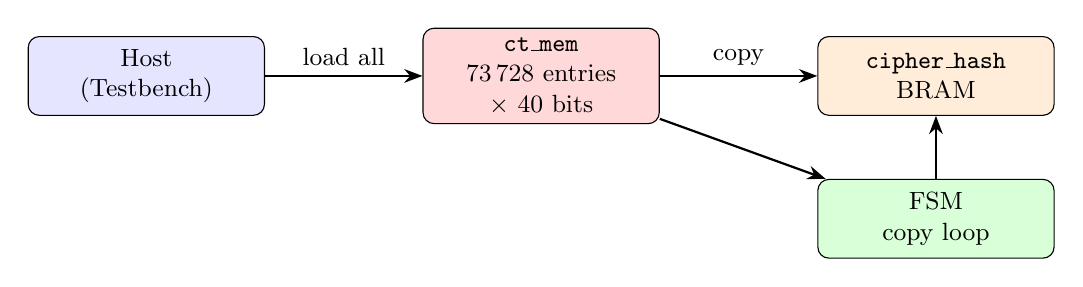
\begin{tikzpicture}[
  box/.style={draw, rounded corners, minimum width=3cm, minimum height=1cm,
              align=center, font=\small},
  arr/.style={-{Stealth}, thick},
  node distance=1.2cm and 2.0cm
]
  \node[box, fill=blue!10]  (host)   {Host\\(Testbench)};
  \node[box, fill=red!15,   right=2cm of host]  (ctmem)  {\texttt{ct\_mem}\\73\,728 entries\\$\times$ 40 bits};
  \node[box, fill=orange!15,right=2cm of ctmem] (ch)     {\texttt{cipher\_hash}\\BRAM};
  \node[box, fill=green!15, below=0.8cm of ch]  (fsm)    {FSM\\copy loop};

  \draw[arr] (host)  -- node[above]{\small load all} (ctmem);
  \draw[arr] (ctmem) -- node[above]{\small copy} (ch);
  \draw[arr] (fsm)   -- (ch);
  \draw[arr] (ctmem) -- (fsm);
\end{tikzpicture}
\caption{Original architecture: host loads all ciphertexts into
\texttt{ct\_mem}; the FSM then copies each to \texttt{cipher\_hash} before
computing.}
\label{fig:orig_arch}
\end{figure}

\subsection{Internal Buffer: \texttt{ct\_mem}}

The buffer was declared as a flat array:

\begin{lstlisting}[caption={Original \texttt{ct\_mem} declaration in \texttt{hash\_verifier.v}.}]
(* ram_style = "block" *)
reg [Q_WIDTH-1:0] ct_mem [0:73727];
// 3 ciphertexts x CT_SIZE slots x N coefficients
// = 3 x 3 x 8192 = 73,728 entries x 40 bits
\end{lstlisting}

The array was addressed by a linear function:
\[
  \text{addr} = \text{ct\_id} \times \texttt{CT\_SIZE} \times N
              + \text{comp} \times N + \text{coeff\_index}
\]

\subsection{Original FSM Protocol}

The original finite state machine used a single \texttt{start} pulse
after all three ciphertexts were loaded:

\begin{enumerate}
  \item Host writes $\mathbf{c}_1$, $\mathbf{c}_2$, $\mathbf{c}_3$
        into \texttt{ct\_mem} (identified by \texttt{ct\_id} port).
  \item Assert \texttt{start} once.
  \item FSM enters \texttt{ST\_LOAD\_C1}: copies $\mathbf{c}_1$ from
        \texttt{ct\_mem} $\rightarrow$ \texttt{cipher\_hash} BRAM
        ($\texttt{CT\_SIZE} \times N$ cycles).
  \item \texttt{cipher\_hash} computes $h_1$.
  \item FSM enters \texttt{ST\_LOAD\_C2}: copies $\mathbf{c}_2$
        ($\texttt{CT\_SIZE} \times N$ cycles).
  \item \texttt{cipher\_hash} computes $h_2$.
  \item FSM enters \texttt{ST\_LOAD\_C3}: copies $\mathbf{c}_3$
        ($\texttt{CT\_SIZE} \times N$ cycles).
  \item \texttt{cipher\_hash} computes $h_3$.
  \item Verify $h_3 = h_1 \cdot h_2 + h_2$; assert \texttt{done}.
\end{enumerate}

\subsection{BRAM Utilisation Before Optimisation}

The BRAM usage is summarised in Table~\ref{tab:bram_before}.

\begin{table}[h]
\centering
\begin{tabular}{lrr}
\toprule
\textbf{Source} & \textbf{BRAM36 used} & \textbf{Calculation} \\
\midrule
\texttt{ct\_mem} (hash\_verifier) & 144 & $\lceil 73728 / 512 \rceil$ \\
\texttt{cipher\_hash} internal RAMs & $\approx 72$ & $h_1, h_2, h_3$, ct, $r$ \\
\texttt{poly\_mul} / \texttt{ntt} & $\approx 164$ & NTT working buffers \\
\midrule
\textbf{Total} & $\mathbf{\approx 380}$ & \\
\midrule
\textbf{Available (xc7a200t)} & $\mathbf{365}$ & \\
\bottomrule
\end{tabular}
\caption{BRAM36 utilisation before optimisation. The design exceeded
the device limit by $\approx 15$ tiles, causing a DRC UTLZ-1 error.}
\label{tab:bram_before}
\end{table}

The synthesis tool (Vivado 2025.2) reported:
\begin{center}
\texttt{[DRC UTLZ-1] BRAM resource over-usage: 380 BRAMs used,
365 available on xc7a200t.}
\end{center}

% ================================================================
\section{Problem Analysis}
\label{sec:problem}

\subsection{Root Cause: Redundant Buffering}

The \texttt{ct\_mem} buffer was logically redundant. Its purpose was
to hold all three ciphertexts while the FSM sequentially copied each
one into the \texttt{cipher\_hash} internal BRAM. However,
\texttt{cipher\_hash} already contains its own BRAM for ciphertext
storage. The copy loops therefore consumed:

\begin{itemize}
  \item \textbf{144 BRAM36 tiles} for storage that existed nowhere else to
        be: the same data was immediately re-written into
        \texttt{cipher\_hash}'s own BRAM.
  \item \textbf{Wasted cycles}: $3 \times \texttt{CT\_SIZE} \times N
        = 3 \times 3 \times 8192 = 73{,}728$ copy cycles per
        verification, before any computation began.
\end{itemize}

\subsection{Why the Buffer Existed}

The original design was built around a ``bulk-load then compute''
protocol: the host delivers all ciphertexts at once (identified by a
\texttt{ct\_id} port), and the FSM manages the sequencing internally.
This approach is simple to drive from the host but requires the module
to retain all inputs simultaneously — hence the buffer.

% ================================================================
\section{Optimisation: 3-Phase Sequential Load Protocol}
\label{sec:optimisation}

\subsection{Key Insight}

The three hash computations $h_1$, $h_2$, $h_3$ are sequential: only
one is active at a time. \texttt{cipher\_hash}'s internal BRAM is
therefore idle during the two phases it is not computing. The host can
load the next ciphertext into that idle BRAM directly, eliminating the
need for any intermediate storage.

\subsection{Changes Made}

\subsubsection{Removed from \texttt{hash\_verifier.v}}
\begin{itemize}
  \item \texttt{ct\_mem[0:73727]} array ($-144$ BRAM36 tiles)
  \item \texttt{ct\_lin()} addressing function
  \item \texttt{ct\_id} input port
  \item FSM states \texttt{ST\_LOAD\_C1}, \texttt{ST\_LOAD\_C2},
        \texttt{ST\_LOAD\_C3}
  \item Intermediate copy registers \texttt{ch\_ct\_wr\_*}
\end{itemize}

\subsubsection{Added to \texttt{hash\_verifier.v}}
\begin{itemize}
  \item \texttt{ready} output wire (indicates module is idle and
        ready to accept the next ciphertext load)
  \item FSM states \texttt{ST\_WAIT\_C2}, \texttt{ST\_WAIT\_C3}
  \item Direct wiring: \texttt{ct\_wr\_*} ports pass straight through
        to \texttt{cipher\_hash}
\end{itemize}

\subsubsection{New \texttt{ready} Signal}

\begin{lstlisting}[caption={Ready signal assignment in \texttt{hash\_verifier.v}.}]
assign ready = (state == ST_IDLE   ||
                state == ST_WAIT_C2 ||
                state == ST_WAIT_C3);
\end{lstlisting}

\texttt{ready = 1} means the host may safely write the next
ciphertext. \texttt{ready = 0} means \texttt{cipher\_hash} is
computing and the BRAM must not be overwritten.

\subsubsection{New FSM State Diagram}

Table~\ref{tab:fsm} lists the FSM states after optimisation.

\begin{table}[h]
\centering
\begin{tabular}{lll}
\toprule
\textbf{State} & \textbf{Action} & \textbf{ready} \\
\midrule
\texttt{ST\_IDLE}     & Wait for $\mathbf{c}_1$ load + \texttt{start} & 1 \\
\texttt{ST\_HASH\_C1} & \texttt{cipher\_hash} computes $h_1$           & 0 \\
\texttt{ST\_SAVE\_H1} & Drain $h_1$ result to \texttt{h1[]} BRAM       & 0 \\
\texttt{ST\_WAIT\_C2} & Wait for $\mathbf{c}_2$ load + \texttt{start}  & 1 \\
\texttt{ST\_HASH\_C2} & \texttt{cipher\_hash} computes $h_2$           & 0 \\
\texttt{ST\_SAVE\_H2} & Drain $h_2$ result to \texttt{h2[]} BRAM       & 0 \\
\texttt{ST\_WAIT\_C3} & Wait for $\mathbf{c}_3$ load + \texttt{start}  & 1 \\
\texttt{ST\_HASH\_C3} & \texttt{cipher\_hash} computes $h_3$           & 0 \\
\texttt{ST\_SAVE\_H3} & Drain $h_3$ result to \texttt{h3[]} BRAM       & 0 \\
\texttt{ST\_LOAD\_MUL}& Load $h_1$, $h_2$ into \texttt{poly\_mul}      & 0 \\
\texttt{ST\_WAIT\_MUL}& Wait for $h_1 \cdot h_2$                       & 0 \\
\texttt{ST\_LOAD\_ADD}& Load result + $h_2$ into \texttt{poly\_add}    & 0 \\
\texttt{ST\_WAIT\_ADD}& Wait for $h_1 h_2 + h_2$                       & 0 \\
\texttt{ST\_COMPARE}  & Compare expected vs $h_3$ coefficient-wise      & 0 \\
\texttt{ST\_DONE}     & Assert \texttt{done} and \texttt{valid}         & 0 \\
\bottomrule
\end{tabular}
\caption{FSM states after optimisation. States where \texttt{ready = 1}
are the windows in which the host loads the next ciphertext.}
\label{tab:fsm}
\end{table}

\subsection{New Host Protocol}

The host must follow the 3-phase sequential protocol shown in
Listing~\ref{lst:protocol}.

\begin{lstlisting}[language=Verilog,
  caption={3-phase load protocol (from \texttt{tb\_hash\_verifier.v}).},
  label={lst:protocol}]
// Phase 1: load c1, trigger h1 computation
load_ct_component(2'd0, c1_comp0);  // 8192 writes
load_ct_component(2'd1, c1_comp1);  // 8192 writes
start = 1; @(posedge clk); start = 0;
while (!ready) @(posedge clk);      // wait for h1 done

// Phase 2: load c2, trigger h2 computation
load_ct_component(2'd0, c2_comp0);
load_ct_component(2'd1, c2_comp1);
start = 1; @(posedge clk); start = 0;
while (!ready) @(posedge clk);      // wait for h2 done

// Phase 3: load c3, trigger h3 + verify
load_ct_component(2'd0, c3_comp0);
load_ct_component(2'd1, c3_comp1);
load_ct_component(2'd2, c3_comp2);
start = 1; @(posedge clk); start = 0;
while (!done) @(posedge clk);       // wait for verification
\end{lstlisting}

\subsection{New Architecture}

Figure~\ref{fig:new_arch} shows the optimised data flow. No
intermediate buffer exists; ciphertext data flows directly from the
host into \texttt{cipher\_hash}'s own BRAM.

\begin{figure}[h]
\centering
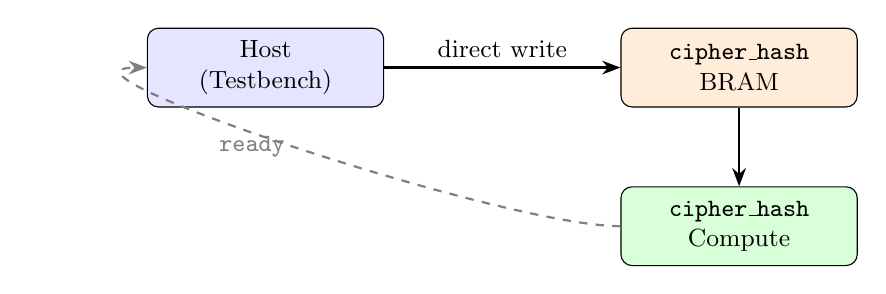
\begin{tikzpicture}[
  box/.style={draw, rounded corners, minimum width=3cm, minimum height=1cm,
              align=center, font=\small},
  arr/.style={-{Stealth}, thick},
  darr/.style={-{Stealth}, thick, dashed, gray},
  node distance=1.2cm and 2.5cm
]
  \node[box, fill=blue!10]    (host) {Host\\(Testbench)};
  \node[box, fill=orange!15, right=3cm of host] (ch) {\texttt{cipher\_hash}\\BRAM};
  \node[box, fill=green!15,  below=1cm of ch]   (comp) {\texttt{cipher\_hash}\\Compute};

  \draw[arr]  (host) -- node[above]{\small direct write} (ch);
  \draw[arr]  (ch)   -- (comp);
  \draw[darr] (comp.west) .. controls +(-1.5,0) and +(-1.5,0) ..
              node[left]{\small \texttt{ready}} (host.west);
\end{tikzpicture}
\caption{Optimised architecture: host writes directly into
\texttt{cipher\_hash} BRAM. The \texttt{ready} signal tells the host
when the next load window opens.}
\label{fig:new_arch}
\end{figure}

% ================================================================
\section{Results}
\label{sec:results}

\subsection{BRAM Utilisation}

\begin{table}[h]
\centering
\begin{tabular}{lrr}
\toprule
\textbf{Metric} & \textbf{Before} & \textbf{After} \\
\midrule
\texttt{ct\_mem} BRAM36 tiles & 144 & 0 \\
Other BRAM36 tiles & $\approx 236$ & $\approx 236$ \\
\textbf{Total BRAM36} & $\mathbf{\approx 380}$ & $\mathbf{\approx 236}$ \\
Available (xc7a200t) & 365 & 365 \\
\textbf{Over limit?} & \textbf{Yes (+15)} & \textbf{No ($-129$)} \\
\bottomrule
\end{tabular}
\caption{BRAM utilisation before and after optimisation.}
\label{tab:bram_after}
\end{table}

Removing \texttt{ct\_mem} freed \textbf{144 BRAM36 tiles}, reducing
total usage from $\approx 380$ to $\approx 236$ --- comfortably within
the 365-tile device limit.

\subsection{Simulation Results}

Behavioural simulation was run in Vivado 2025.2 using test vectors
generated by \texttt{gen\_test\_vectors.py}. Results are shown in
Table~\ref{tab:sim}.

\begin{table}[h]
\centering
\begin{tabular}{lrr}
\toprule
\textbf{Metric} & \textbf{Before} & \textbf{After} \\
\midrule
Simulation result & PASS (valid=1) & PASS (valid=1) \\
Total simulation cycles & $\approx 8{,}300{,}000$ & $5{,}472{,}357$ \\
Cycles saved & --- & $\approx 2{,}827{,}643$ \\
Cycle reduction & --- & $\approx 34\%$ \\
\bottomrule
\end{tabular}
\caption{Simulation results before and after optimisation.}
\label{tab:sim}
\end{table}

The Vivado simulation log confirmed correctness:

\begin{verbatim}
================================================================
  PASS - valid = 1
  H(c3) == H(c1)*H(c2) + H(c2) verified in hardware!
  Total simulation cycles: 5472357
================================================================
\end{verbatim}

\subsection{Cycle Savings Breakdown}

The $\approx 2.8$M cycle reduction comes from eliminating the three
internal copy loops that transferred data from \texttt{ct\_mem} to
\texttt{cipher\_hash}:
\[
  \text{Saved} = 3 \times \texttt{CT\_SIZE} \times N
               = 3 \times 3 \times 8192 = 73{,}728 \text{ copy cycles}
\]
The remaining savings reflect pipeline and FSM overhead that was
removed along with the copy states.

% ================================================================
\section{Trade-offs}
\label{sec:tradeoffs}

\begin{table}[h]
\centering
\begin{tabular}{p{5cm} p{4.5cm} p{4.5cm}}
\toprule
\textbf{Aspect} & \textbf{Before} & \textbf{After} \\
\midrule
Host protocol & Load all 3 then single \texttt{start} &
  3-phase: load one, \texttt{start}, wait \texttt{ready}, repeat \\
\midrule
Host complexity & Simple: one burst load & Slightly more: must honour
  \texttt{ready} handshake between phases \\
\midrule
Module responsibility & Internally sequences all copies &
  Host responsible for interleaving loads and computation \\
\midrule
BRAM usage & $\approx 380$ (over device limit) & $\approx 236$
  (fits comfortably) \\
\midrule
Cycle count & $\approx 8.3$M & $5.47$M \\
\bottomrule
\end{tabular}
\caption{Trade-off comparison.}
\label{tab:tradeoffs}
\end{table}

The main cost of the optimisation is that the host must now participate
in the sequencing (observing \texttt{ready} between phases). This is a
standard handshake pattern in hardware interfaces and does not add
significant complexity.

% ================================================================
\section{Conclusion}
\label{sec:conclusion}

Optimisation 1 eliminated the 144-BRAM \texttt{ct\_mem} internal
ciphertext buffer from \texttt{hash\_verifier} by changing the loading
protocol from a single bulk-load to a 3-phase sequential scheme. The
key observations were:

\begin{enumerate}
  \item \texttt{cipher\_hash} already owns a BRAM for ciphertext
        storage; \texttt{ct\_mem} was a redundant copy.
  \item The three hash computations are sequential, so the host can
        load each ciphertext directly into the shared \texttt{cipher\_hash}
        BRAM one at a time, reusing the same storage.
  \item Removing the copy loop FSM states also eliminated 73\,728
        wasted cycles per verification.
\end{enumerate}

The design now fits on the Xilinx xc7a200t device (236 of 365
BRAM36 tiles used) and simulation confirms correctness
(\texttt{valid = 1}) with a 34\% reduction in total cycle count.

\subsection*{Next Steps}

\begin{description}
  \item[Step 2] Use both BRAM read ports for NTT butterfly computation
        inside \texttt{ntt.v}, reducing butterfly latency and improving
        maximum clock frequency.
  \item[Step 4] Parallel RNS: instantiate three \texttt{poly\_mul}
        cores simultaneously, one per prime modulus, targeting a
        $3\times$ throughput improvement on the polynomial
        multiplication pipeline.
\end{description}

\end{document}
